%        File: pres.tex
%     Created: Tues June 19 07:00 AM 2012 C
%
%\documentclass[11pt,handout]{beamer}
\documentclass[9pt]{beamer}
% for beamer arrows
\usepackage{tikz}
\usetikzlibrary{arrows,shapes}



\usepackage{graphicx}
\usepackage{booktabs} % nice rules for tables
\usepackage{microtype} % if using PDF
\usepackage{bigints}
\newcommand{\units}[1] {\:\text{#1}}%
\newcommand{\SN}{S$_N$}%{S$_\text{N}$}%{$S_N$}%
\DeclareMathOperator{\erf}{erf}
\setbeamertemplate{caption}[numbered]

\usetheme[white]{Wisconsin}
%\title[short title]{long title}
\title[Cyclus and Cyder]{ Cyclus and Cyder : Open Source Tools for Fuel Cycle and Repository Analysis}
\title[Key Disposal Processes and Parameters]{ Key Processes and Parameters in a Generic Clay Disposal System Model}
%\subtitle[short subtitle]{long subtitle}
\subtitle[ANS2012]{2012 American Nuclear Society Winter Meeting, San Diego} 
%\author[short name]{long name}
\author[Kathryn Huff]{Kathryn D.~Huff$^{1,2}$ \& W. Mark Nutt$^2$}
%\date[short date]{long date}
\date[11.13.2012]{November 13, 2012}
%\institution[short name]{long name}
\institute[UW-Madison]{$^1$University of Wisconsin-Madison \& $^2$Argonne National Laboratory}
%page numbers
\setbeamertemplate{footline}[page number]
%Those icons in the references are terrible looking
\setbeamertemplate{bibliography item}[text]

%%%%%%%%%%%%%%%%%%%%%%%%%%%%%%%%%%%%%%%%%%%%%%%%%%%%%%%%%%%%%
\usepackage[acronym,toc]{glossaries}
\include{acros}
\makeglossaries


\begin{document}
%%%%%%%%%%%%%%%%%%%%%%%%%%%%%%%%%%%%%%%%%%%%%%%%%%%%%%%%%%%%%
%% From uw-beamer Here's a handy bit of code to place at 
%% the beginning of your presentation (after \begin{document}):
\newcommand*{\alphabet}{ABCDEFGHIJKLMNOPQRSTUVWXYZabcdefghijklmnopqrstuvwxyz}
\newlength{\highlightheight}
\newlength{\highlightdepth}
\newlength{\highlightmargin}
\setlength{\highlightmargin}{2pt}
\settoheight{\highlightheight}{\alphabet}
\settodepth{\highlightdepth}{\alphabet}
\addtolength{\highlightheight}{\highlightmargin}
\addtolength{\highlightdepth}{\highlightmargin}
\addtolength{\highlightheight}{\highlightdepth}
\newcommand*{\Highlight}{\rlap{\textcolor{HighlightBackground}{\rule[-\highlightdepth]{\linewidth}{\highlightheight}}}}
%%%%%%%%%%%%%%%%%%%%%%%%%%%%%%%%%%%%%%%%%%%%%%%%%%%%%%%%%%%%%
%%--------------------------------%%
\frame{
\titlepage
}
%%--------------------------------%%
\AtBeginSection[]{
\begin{frame}[c]
  \frametitle{Outline}
  \tableofcontents[currentsection]
\end{frame}
}

%%--------------------------------%%
%%--------------------------------%%

%%%%%%%%%%%%%%%%%%%%%%%%%%%%%%%%%%%%%%%%%%%%%%%%%%%%%%%%%%%%%%%%%%%%%%%%%%%%%%%%
  
\section{Introduction}
\begin{frame}[c]
  \frametitle{Clay Generic Disposal System Model}
Sensitivity analysis based on the detailed computational \textbf{Clay 
  \gls{GDSM}} developed by the \gls{UFD} campaign \cite{clayton_generic_2011}.  
  was performed with respect to various \textbf{key processes and parameters} 
  affecting long-term post-closure performance of geologic repositories in 
  \textbf{clay} media.

\end{frame}

\begin{frame}[c]
  \frametitle{Clay Generic Disposal System Model}
     \begin{figure}[h!]
         \includegraphics[width=.4\textwidth]{belgianClayRedImp.eps}
         \caption{Belgian reference concept in Boom Clay 
         \cite{von_lensa_red-impact_2008}.}
     \end{figure}
     \begin{figure}[h!]
         \includegraphics[width=0.4\textwidth]{clayGonzales.eps}
         \caption{U.S. Clay Deposits, ref. \cite{gonzales_shales_1985}.}
     \end{figure}
   \hspace{0.01cm}
\end{frame}



\begin{frame}[c]
  \frametitle{Clay Generic Disposal System Model}
The Clay \gls{GDSM}, developed at Argonne National Lab, is built on the GoldSim 
simulation framework and contaminant transport model.  It simulates chemical and 
physical attenuation processes \cite{golder_goldsim_2010, 
golder_goldsim_ct_2010}, including 
\begin{itemize}
  \item  chemical and physical attenuation processes including
  \item radionuclide solubility,
  \item dispersion phenomena,
  \item and reversible sorption.
\end{itemize}

Input parameters include 
\begin{itemize}
  \item geometry specifications (e.g. repository depth),
  \item geologic material properties (e.g. clay porosity), 
  \item geochemical data (e.g. elemental solubility limits),
  \item and environmental parameters (e.g. natural system velocity). 
\end{itemize}
\end{frame}

\begin{frame}[c]
  \frametitle{Clay Generic Disposal System Model}
  \vspace{2cm}
\begin{figure}[h!]
\includegraphics[width=0.6\textwidth]{feps.eps}
\caption{General Features Events and Processes in the Clay repository model 
  \ref{clayton_generic_2011}.}
\end{figure}
\end{frame}

\begin{frame}[c]
  \frametitle{Clay Generic Disposal System Model}
The disposal concept modeled by the Clay \gls{GDSM} \cite{nutt_generic_2009} is
\begin{itemize}
  \item an array of spent nuclear fuel packages 
  \item emplaced horizontally
  \item in excavated tunnels, 
  \item backfilled by a reducing bentonite clay,
  \item within a clay repository environment, 
  \item \textbf{500 meters} beneath the earth's surface.
\end{itemize}
\end{frame}

\begin{frame}[c]
  \frametitle{Mean of the Peak Annual Dose}
In this analysis, repository performance is quantified by radiation dose to a 
hypothetical receptor. Specifically, the mean of the peak annual dose,

\footnotesize{
  \begin{align} \label{MoP}
    D_{MoP,i} &= \frac{\sum_{r=1}^{N}{\max\left[\left.D_{r,i}(t)\right|_{\forall t}\right]}}{N}
    \intertext{where}
    D_{MoP,i} &= \mbox{ mean of peak annual dose due to isotope i } [mrem/yr]\nonumber\\
    D_{r,i}(t) &= \mbox{ year t dose in realization r due to isotope i } [mrem/yr]\nonumber\\
    N &= \mbox{number of realizations, } \nonumber
\end{align}
}

is a conservative metric of repository performance and should not be confused 
with the peak of the mean annual dose.

\footnotesize{
  \begin{align} \label{PoM}
    D_{PoM,i} &= \max\left[{\frac{\sum_{r=1}^{N}{\left.D_{r,i}(t)\right|_{\forall t}}}{N}}\right]\\
              &= \mbox{peak of the mean annual dose due to isotope i } [mrem/yr].\nonumber
  \end{align}
}
\end{frame}

\begin{frame}[c]
  \frametitle{Sampling Strategy}
  \footnotesize{
To develop a many dimensional overview, both individual and dual parametric cases were performed.

\begin{itemize}
  \item \textbf{Individual parameter cases} varied a single parameter of interest in 
detail over a broad range of values. 
  \item \textbf{Dual parameter cases} were performed for pairs of parameters expected to exhibit some covariance. 
\end{itemize}    
For each case, forty simulation 
groups varied the parameter or parameters within the range considered. 
For each simulation group, a 100 realization simulation was completed 
\cite{clayton_generic_2011, 
nutt_generic_2009}.  

\begin{table}[ht!]
\centering
\footnotesize{
\begin{tabular}{|l|l|l|r|r|}
\multicolumn{5}{c}{\textbf{Simulation Cases}}\\
\hline
\textbf{Case} & \textbf{Parameter} & \textbf{Units} & \textbf{Min. Value} & \textbf{Max. Value}\\
\hline
II    & $V_{adv, y}$ & $[m \cdot yr^{-1}]$       & $6.31\times10^{-8}$  &  $6.31\times10^{-4}$ \\
      & $D_{eff}$    & $[m^2\cdot s^{-1}]$       & $10^{-8}$    &  $10^{-5}$ \\
\hline
\end{tabular}
\caption{Case II varied the advective velocity and effective diffusivity to 
  determine the nature of the threshold between the diffusive and advective 
  regimes. This dual parameter simulation case had 40 simulation 
groups of 100 realizations each.}
\label{tab:Cases}
}
\end{table}


}

\end{frame}


%%%%%%%%%%%%%%%%%%%%%%%%%%%%%%%%%%%%%%%%%%%%%%%%%%%%%%%%%%%%%%%%%%%%%%%%%%%%%%%%
  
\begin{frame}[c]
  \frametitle{Case I : Diffusion Coefficient and Inventory}
The sensitivity of the peak dose to the reference diffusivity of the 
host rock was analyzed. 
That is, the radionuclide inventory in a reference \gls{MTHM} of commercial spent nuclear fuel was multiplied by a scalar mass factor.  
It was expected that changing these two parameters in tandem would capture 
\begin{itemize}
  \item the importance of diffusivity in the far field 
  \item a threshold at which the effect of waste inventory dissolution is attenuated by solubility limits.
\end{itemize}
\end{frame}

\begin{frame}[c]
  \frametitle{Case I : Diffusion Coefficient and Inventory}
\begin{table}[ht!]
\centering
\footnotesize{
\begin{tabular}{|l|l|l|r|r|}
\multicolumn{5}{c}{\textbf{Simulation Cases}}\\
\hline
\textbf{Case} & \textbf{Parameter} & \textbf{Units} & \textbf{Min. Value} & \textbf{Max. Value}\\
\hline
I     & $D_{eff}$    & $[m^2\cdot s^{-1}]$       & $10^{-8}$    &  $10^{-5}$ \\
      & Inventory              & [MTHM]         & $10^{-4}$    &  $10^1$ \\
\hline
\end{tabular}
\caption{Each dual and single parameter simulation case had 40 simulation 
groups of 100 realizations each.}
\label{tab:Cases}
}
\end{table}


\begin{table}[hbp!]
\centering
\includegraphics[width=0.7\textwidth]{DiffCoeffAndInvEBSFail/DiffCoeffAndInvGroups.eps}
\caption{Diffusion coefficient and mass factor simulation groupings.}
\label{tab:DiffCoeffAndInvGroups}
\end{table}
\end{frame}

\begin{frame}[c]
  \frametitle{Case I : Diffusion Coefficient and Inventory}
\begin{figure}[ht]
\centering
\includegraphics[width=\linewidth]{./DiffCoeffAndInvEBSFail/I-129.eps}
\caption{The peak doses due to highly soluble, non-sorbing elements such as $I$ 
are largely directly proportional to the relative diffusivity.  }
\label{fig:DCInvI129}
\end{figure}
\end{frame}

\begin{frame}[c]
  \frametitle{Case I : Diffusion Coefficient and Inventory}
\begin{figure}[ht]
\centering
\includegraphics[width=\linewidth]{DiffCoeffAndInvEBSFail/I-129-MF.eps}
\caption{$^{129}I$ mass factor sensitivity.}
\caption{The peak doses due to highly soluble, non-sorbing elements such as $I$ 
are  proportional to the radionuclide inventory.}
\label{fig:DCInvI129MF}
\end{figure}
\end{frame}

\begin{frame}[c]
  \frametitle{Case I : Diffusion Coefficient and Inventory}

\begin{figure}[ht]
\centering
\includegraphics[width=\linewidth]{DiffCoeffAndInvEBSFail/Cl-36.eps}
\caption{The peak doses due to highly soluble, non-sorbing elements such as $Cl$ 
are largely directly proportional to the relative diffusivity.  }
\label{fig:DCInvCl36}
\end{figure}
\end{frame}

\begin{frame}[c]
  \frametitle{Case I : Diffusion Coefficient and Inventory}

\begin{figure}[ht]
\centering
\includegraphics[width=\linewidth]{DiffCoeffAndInvEBSFail/Cl-36-MF.eps}
\caption{The peak doses due to highly soluble, non-sorbing elements such as $I$ 
are  proportional to the radionuclide inventory.}
\label{fig:DCInvCl36MF}
\end{figure}
\end{frame}


\begin{frame}[c]
  \frametitle{Case I : Diffusion Coefficient and Inventory}
\begin{figure}[ht!]
\centering
\includegraphics[width=\linewidth]{DiffCoeffAndInvEBSFail/Tc-99.eps}
\caption{$^{99}Tc$ relative diffusivity sensitivity.} 
\label{fig:DCInvTc99}
\end{figure}
\end{frame}

\begin{frame}[c]
  \frametitle{Case I : Diffusion Coefficient and Inventory}

\begin{figure}[ht!]
\centering
\includegraphics[width=\linewidth]{DiffCoeffAndInvEBSFail/Tc-99-MF.eps}
\caption{$^{99}Tc$ mass factor sensitivity.}
\label{fig:DCInvTc99MF}
\end{figure}
\end{frame}

\begin{frame}[c]
  \frametitle{Case I : Diffusion Coefficient and Inventory}


\begin{figure}[ht!]
\centering
\includegraphics[width=\linewidth]{DiffCoeffAndInvEBSFail/Np-237.eps}
\caption{$^{237}Np$ relative diffusivity sensitivity.} 
\label{fig:DCInvNp237}
\end{figure}
\end{frame}

\begin{frame}[c]
  \frametitle{Case I : Diffusion Coefficient and Inventory}

\begin{figure}[ht!]
\centering
\includegraphics[width=\linewidth]{DiffCoeffAndInvEBSFail/Np-237-MF.eps}
\caption{$^{237}Np$ mass factor sensitivity.}
\label{fig:DCInvNp237MF}
\end{figure}
\end{frame}

\begin{frame}[c]
  \frametitle{Case II : Vertical Advective Velocity and Diffusion Coefficient}
Advection is transport driven by bulk water velocity while diffusion is the 
result of Brownian motion across concentration gradients.  The method by which 
the dominant solute transport mode (diffusive or advective) is determined for a 
particular porous medium is by use of the dimensionless Peclet number, 

\begin{align} 
  Pe &= \frac{nvL}{\alpha nv + D_{eff}},\\
  &= \frac{\mbox{advective rate}}{\mbox{diffusive rate}}\nonumber
  \intertext{where} 
  n &= \mbox{ solute accessible porosity } [\%]\nonumber\\
  v &= \mbox{ advective velocity } [m\cdot s^{-1}] \nonumber\\
  L &= \mbox{ transport distance } [m]\nonumber\\
  \alpha &= \mbox{ dispersivity } [m]\nonumber\\
  D_{eff} &= \mbox{ effective diffusion coefficient } [m^2\cdot s^{-1}].\nonumber
\end{align}
For a high $Pe$ number, advection is the dominant transport mode, while 
diffusive or dispersive transport dominates for a low $Pe$ number
\cite{schwartz_fundamentals_2004}.
\end{frame}

\begin{frame}[c]
  \frametitle{Case II : Vertical Advective Velocity and Diffusion Coefficient}
  \begin{table}[ht!]
\centering
\footnotesize{
\begin{tabular}{|l|l|l|r|r|}
\multicolumn{5}{c}{\textbf{Simulation Cases}}\\
\hline
\textbf{Case} & \textbf{Parameter} & \textbf{Units} & \textbf{Min. Value} & \textbf{Max. Value}\\
\hline
II    & $V_{adv, y}$ & $[m \cdot yr^{-1}]$       & $6.31\times10^{-8}$  &  $6.31\times10^{-4}$ \\
      & $D_{eff}$    & $[m^2\cdot s^{-1}]$       & $10^{-8}$    &  $10^{-5}$ \\
\hline
\end{tabular}
\caption{Case II varied the advective velocity and effective diffusivity to 
  determine the nature of the threshold between the diffusive and advective 
  regimes. This dual parameter simulation case had 40 simulation 
groups of 100 realizations each.}
\label{tab:Cases}
}
\end{table}



The forty runs are a combination of the five values of the vertical advective 
velocity and eight magnitudes of relative diffusivity.
\begin{table}
\centering
\includegraphics[width=0.8\textwidth]{AdvVelAndDiffCoeffEBSFail/AdvVelAndDiffCoeffGroups.eps}
\caption{Vertical advective velocity and diffusion coefficient simulation groupings.}
\label{tab:AdvVelAndDiffCoeffGroups}
\end{table}
\end{frame}

\begin{frame}[c]
  \frametitle{Case II : Vertical Advective Velocity and Diffusion Coefficient}
\begin{figure}[htp!]
\centering
\includegraphics[width=0.8\textwidth]{AdvVelAndDiffCoeffEBSFail/I-129.eps}
\caption{$^{129}I$. For vertical advective velocities 
$6.31\times10^{-6}[m/yr]$ and above, lower reference diffusivities are 
ineffective at attenuating the mean of the peak doses for soluble, non-sorbing 
elements. 
}
\label{fig:VAdvVelI129}
\end{figure}
\end{frame}

\begin{frame}[c]
  \frametitle{Case II : Vertical Advective Velocity and Diffusion Coefficient}

\begin{figure}[ht!]
\centering
\includegraphics[width=0.8\textwidth]{AdvVelAndDiffCoeffEBSFail/I-129-VAdvVel.eps}
\caption{$^{129}I$.
For vertical advective velocities 
$6.31\times10^{-6}[m/yr]$ and above, lower reference diffusivities are 
ineffective at attenuating the mean of the peak doses for soluble, non-sorbing 
elements. 
}
\label{fig:VAdvVelI129VAdvVel}
\end{figure}
\end{frame}

\begin{frame}[c]
  \frametitle{Case II : Vertical Advective Velocity and Diffusion Coefficient}
\begin{figure}[htp!]
\centering
\includegraphics[width=0.8\textwidth]{AdvVelAndDiffCoeffEBSFail/Np-237.eps}
\caption{$^{237}Np$.
shows a very weak influence on peak annual dose 
rate for low reference diffusivities, but a direct proportionality between 
dose and reference diffusivity above a threshold.}
\label{fig:VAdvVelNp237}
\end{figure}
\end{frame}

\begin{frame}[c]
  \frametitle{Case II : Vertical Advective Velocity and Diffusion Coefficient}
\begin{figure}[ht!]
\centering
\includegraphics[width=0.8\textwidth]{AdvVelAndDiffCoeffEBSFail/Np-237-VAdvVel.eps}
\caption{$^{237}Np$.
shows a very weak influence on peak annual dose 
rate for low reference diffusivities, but a direct proportionality between 
dose and reference diffusivity above a threshold.}
\label{fig:VAdvVelNp237VAdvVel}
\end{figure}
\end{frame}

\begin{frame}[c]
  \frametitle{Case II : Vertical Advective Velocity and Diffusion Coefficient}
\begin{figure}[htp!]
\centering
\includegraphics[width=0.8\textwidth]{AdvVelAndDiffCoeffEBSFail/Se-79.eps}
\caption{$^{79}Se$.
$Se$ is non sorbing, but solubility limited.  
For low vertical advective velocity, 
the system is diffusion dominated.}
\label{fig:VAdvVelSe79}
\end{figure}
\end{frame}

\begin{frame}[c]
  \frametitle{Case II : Vertical Advective Velocity and Diffusion Coefficient}
\begin{figure}[ht!]
\centering
\includegraphics[width=0.8\textwidth]{AdvVelAndDiffCoeffEBSFail/Se-79-VAdvVel.eps}
\caption{$^{79}Se$.
$Se$ is non sorbing, but solubility limited.  
For high vertical advective 
velocity, the diffusivity remains important even in the advective regime as 
spreading facilitates transport in the presence of solubility limited transport. 
vertical advective velocity sensitivity.}
\label{fig:VAdvVelSe79VAdvVel}
\end{figure}
\end{frame}



\begin{frame}[c]
  \frametitle{Case III : Solubility Coefficient}
The reference solubilities for each element were multiplied by the multiplier 
for each simulation group. This technique preserved relative solubility among 
  elements. 

\begin{table}[ht!]
\centering
\footnotesize{
\begin{tabular}{|l|l|l|r|r|}
\multicolumn{5}{c}{\textbf{Simulation Cases}}\\
\hline
\textbf{Case} & \textbf{Parameter} & \textbf{Units} & \textbf{Min. Value} & \textbf{Max. Value}\\
\hline
III   & $S_i$        & $[mol\cdot m^{-3}]$       & $(1\times10^{-9})\langle S_i\rangle $    &  $(5\times10^{10})\langle S_i\rangle $ \\
\hline
\end{tabular}
\caption{Case III varied a solubility factor across many magnitudes. This single parameter simulation case had 40 simulation 
groups of 100 realizations each.}
\label{tab:Cases}
}
\end{table}


\end{frame}

\begin{frame}[c]
  \frametitle{Case III : Solubility Coefficient}


\begin{figure}[ht]
\centering
\includegraphics[width=0.8\textwidth]{Solubility/Solubility_Summary_SolFactor.eps}
\caption{
The peak annual dose due to an inventory, $N$, of each isotope.
For solubility constants lower than the inventory threshold, the relationship between peak 
annual dose and solubility limit is strong.}
\label{fig:SolSumFactor}
\end{figure}
\end{frame}



\begin{frame}[c]
  \frametitle{Case IV : Partition Coefficient}

This analysis investigated the peak dose rate contribution from various 
radionuclides to the partition coefficient of those radionuclides. 

The partition or distribution coefficient, $K_d$, relates the amount of contaminant adsorbed into the 
solid phase of the host medium to the amount of contaminant adsorbed into the 
aqueous phase of the host medium. It is a common empirical coefficient used to 
capture the effects of a number of retardation mechanisms. The coefficient 
$K_d$, in units of $[m^3\cdot kg^{-1}]$, is the ratio of the mass of contaminant in the 
solid to the mass of contaminant in the solution.
\end{frame}

\begin{frame}[c]
  \frametitle{Case IV : Partition Coefficient}
The retardation factor, $R_f$, which is the ratio between velocity of water through a 
volume and the velocity of a contaminant through that volume, can be expressed 
in terms of the partition coefficient,

\begin{align}
  R_f &= 1+\frac{\rho_b}{n_e}K_d
  \intertext{where}
  \rho_b &= ~~\mbox{bulk density}[kg\cdot m^{-3}]\nonumber
  \intertext{and}
  n_e &= ~~\mbox{effective porosity of the medium}[\%].\nonumber
\end{align}
\end{frame}

\begin{frame}[c]
  \frametitle{Case IV : Partition Coefficient}

The parameters in this model were all set to the default values except a multiplier 
applied to the partitioning $K_d$ coefficients.
\begin{table}[ht!]
\centering
\footnotesize{
\begin{tabular}{|l|l|l|r|r|}
\multicolumn{5}{c}{\textbf{Simulation Cases}}\\
\hline
\textbf{Case} & \textbf{Parameter} & \textbf{Units} & \textbf{Min. Value} & \textbf{Max. Value}\\
\hline
IV    & $K_{d,i}$    & $[m^3\cdot kg^{-1}]$       & $(1\times10^{-9})\langle K_{d,i}\rangle $    &  $(5\times10^{10})\langle K_{d,i}\rangle $ \\
\hline
\end{tabular}
\caption{Case IV varied the partitioning coefficient, $K_d$, multiplication 
  factor. This single parameter simulation case had 40 simulation 
groups of 100 realizations each.}
\label{tab:Cases}
}
\end{table}


\end{frame}

\begin{frame}[c]
  \frametitle{Case IV : Partition Coefficient}

\begin{figure}[ht]
\centering
\includegraphics[width=0.8\textwidth]{Sorption/Retardation_Summary_kdFactor.eps}
\caption{
For retardation coefficients greater than a threshold, the 
relationship between peak annual dose and retardation coefficient is a strong 
inverse one. }
\label{fig:KdSumFactor}
\end{figure}
\end{frame}

\begin{frame}[c]
  \frametitle{Case IV : Partition Coefficient}

\begin{figure}[ht]
\centering
\includegraphics[width=0.8\textwidth]{Sorption/Retardation_Summary_kd.eps}
\caption{
For retardation coefficients greater than a threshold, the 
relationship between peak annual dose and retardation coefficient is a strong 
inverse one. }
\label{fig:KdSum}
\end{figure}
\end{frame}



\begin{frame}[c]
  \frametitle{Case V : Waste Form Degradation Rate and Inventory}
These runs varied the waste form degradation rate and the waste inventory mass 
factor.  There were forty runs corresponding to eight values of the waste form degradation 
rate and five values of the mass factor.

\begin{table}[ht!]
\centering
\footnotesize{
\begin{tabular}{|l|l|l|r|r|}
\multicolumn{5}{c}{\textbf{Simulation Cases}}\\
\hline
\textbf{Case} & \textbf{Parameter} & \textbf{Units} & \textbf{Min. Value} & \textbf{Max. Value}\\
\hline
V     & $R_{WFDeg.}$           & $[yr^{-1}]$       & $10^{-9}$    &  $10^{-2}$ \\
      & Inventory              & [MTHM]         & $10^{-4}$    &  $10^1$ \\
\hline
\end{tabular}
\caption{Each dual and single parameter simulation case had 40 simulation 
groups of 100 realizations each.}
\label{tab:Cases}
}
\end{table}


\end{frame}

\begin{frame}[c]
  \frametitle{Case V : Waste Form Degradation Rate and Inventory}

Safety indicators for post closure repository performance have been developed by 
the \gls{UFD} campaign which utilize the inventory multiplier that was varied in 
this study \cite{nutt_generic_2009}. These indicators are normalized by a 
normalization factor (100 mrem/yr) recommended by the \gls{IAEA} as the limit to 
``relevant critical members of the public'' \cite{iaea_international_1996}. The functional form for 
this safety indicator for a single waste category, \gls{HLW}, is just 

\begin{align}
SI_{G} &= \left(\frac{\sum_{i=1}^{N}D_{G,i}(I_i, F_{d})}{100mrem/yr}\right)[GWe/yr].
\label{indicator}
\intertext{where}
SI_{G} &= \mbox{Safety indicator for disposal in media type G}[GWe/yr]\nonumber\\
N &= \mbox{Number of key radionuclides considered in this indicator}\nonumber\\
D_{G,i} &= \mbox{Peak dose rate from isotope i in media type G}[mrem/yr]\nonumber\\
F_{d} &= \mbox{Fractional waste form degradation rate}[1/yr].\nonumber
\end{align}
\end{frame}

\begin{frame}[c]
  \frametitle{Case V : Waste Form Degradation Rate and Inventory}
\begin{figure}[ht!]
\centering
\includegraphics[width=0.8\textwidth]{WFDegAndInv/I-129.eps}
\caption{
Highly soluble and non-sorbing $^{129}I$ demonstrates a direct proportionality between dose rate and 
fractional degradation rate until a turnover where other natural system 
parameters dampen transport.} 
\label{fig:WFDegI129}
\end{figure}
\end{frame}

\begin{frame}[c]
  \frametitle{Case V : Waste Form Degradation Rate and Inventory}

\begin{figure}[ht!]
\centering
\includegraphics[width=0.8\textwidth]{WFDegAndInv/I-129-MF.eps}
\caption{
Highly soluble and non-sorbing $^{129}I$ domonstrates a direct 
proportionality to the inventory multiplier.}
\label{fig:WFDegI129MF}
\end{figure}
\end{frame}

\begin{frame}[c]
  \frametitle{Case V : Waste Form Degradation Rate and Inventory}

\begin{figure}[ht!]
\centering
\includegraphics[width=0.8\textwidth]{WFDegAndInv/Cl-36.eps}
\caption{
Highly soluble and non-sorbing $^{36}Cl$ demonstrates a direct proportionality between dose rate and 
fractional degradation rate until a turnover where other natural system 
parameters dampen transport.} 
\label{fig:WFDegCl36}
\end{figure}

\end{frame}

\begin{frame}[c]
  \frametitle{Case V : Waste Form Degradation Rate and Inventory}
\begin{figure}[ht!]
\centering
\includegraphics[width=0.8\textwidth]{WFDegAndInv/Cl-36-MF.eps}
\caption{
Highly soluble and non-sorbing $^{129}I$ domonstrates a direct 
proportionality to the inventory multiplier.}
\label{fig:WFDegCl36MF}
\end{figure}
\end{frame}

\begin{frame}[c]
  \frametitle{Case V : Waste Form Degradation Rate and Inventory}
The peaks for solubility limited, sorbing elements such as $Tc$ and $Np$, on the 
other hand, have a more dramatic turnover.  For very high degradation rates, the 
dependence on mass factor starts to round off due to attenuation by solubility 
limits.


\begin{figure}[ht!]
\centering
\includegraphics[width=0.8\textwidth]{WFDegAndInv/Tc-99.eps}
\caption{
Solubility limited and sorbing $^{99}Tc$ demonstrates a direct proportionality 
to fractional degradation rate until attuation by its solubility limit and other 
natural system parameters. } 
\label{fig:WFDegTc99}
\end{figure}
\end{frame}

\begin{frame}[c]
  \frametitle{Case V : Waste Form Degradation Rate and Inventory}

\begin{figure}[ht!]
\centering
\includegraphics[width=0.8\textwidth]{WFDegAndInv/Tc-99-MF.eps}
\caption{
  Solubility limited and sorbing $^{99}Tc$ demonstrates a direct proportionality 
to fractional degradation rate until attuation by its solubility limit and other 
natural system parameters. } 
\label{fig:WFDegTc99MF}
\end{figure}

\end{frame}

\begin{frame}[c]
  \frametitle{Case V : Waste Form Degradation Rate and Inventory}

\begin{figure}[ht!]
\centering
\includegraphics[width=0.8\textwidth]{WFDegAndInv/Np-237.eps}
\caption{
  Solubility limited and sorbing $^{237}Np$ demonstrates a direct proportionality 
to fractional degradation rate until attuation by its solubility limit and other 
natural system parameters. } 
\label{fig:WFDegNp237}
\end{figure}
\end{frame}

\begin{frame}[c]
  \frametitle{Case V : Waste Form Degradation Rate and Inventory}

\begin{figure}[ht!]
\centering
\includegraphics[width=0.8\textwidth]{WFDegAndInv/Np-237-MF.eps}
\caption{
  Solubility limited and sorbing $^{237}Np$ demonstrates a direct proportionality 
to fractional degradation rate until attuation by its solubility limit and other 
natural system parameters. } 
\label{fig:WFDegNp237MF}
\end{figure}

\end{frame}


\begin{frame}[c]
  \frametitle{Case VI : Waste Package Failure Time and Diffusion Coefficient}

To investigate the effect of the waste package failure time, it was varied over 
five magnitudes from one thousand to ten million years. Simultaneously, the reference 
diffusivity was varied over the eight magnitudes between $1\times10^{-8}$ and 
$1\times10^{-15}$ in order to determine the correlation between increased 
radionuclide mobility and the waste package lifetime. 
\begin{table}[ht!]
\centering
\footnotesize{
\begin{tabular}{|l|l|l|r|r|}
\multicolumn{5}{c}{\textbf{Simulation Cases}}\\
\hline
\textbf{Case} & \textbf{Parameter} & \textbf{Units} & \textbf{Min. Value} & \textbf{Max. Value}\\
\hline 
VI    & $t_{WPFail}$        & $[yr]$         & $10^3$    &  $10^7$ \\
      & $D_{eff}$           & $[m^2\cdot s^{-1}]$       & $10^{-8}$    &  $10^{-5}$ \\
\hline
\end{tabular}
\caption{Case IV simultaneously varied the time of waste package failure and the 
  reference diffusivity. This dual parameter simulation case had 40 simulation 
groups of 100 realizations each.}
\label{tab:Cases}
}
\end{table}


\end{frame}

\begin{frame}[c]
  \frametitle{Case VI : Waste Package Failure Time and Diffusion Coefficient}

For the clay repository, the waste package failure time is entirely irrelevant 
until waste package failure times reach the million or ten million year time 
scale. 

\begin{figure}[ht!]
\centering
\includegraphics[width=0.8\textwidth]{WPFailExtended/I-129.eps}
\caption{$^{129}I$ waste package failure time sensitivity. }
\label{fig:WPFailI129}
\end{figure}
\end{frame}

\begin{frame}[c]
  \frametitle{Case VI : Waste Package Failure Time and Diffusion Coefficient}

\begin{figure}[ht!]
\centering
\includegraphics[width=0.8\textwidth]{WPFailExtended/I-129-WPFail.eps}
\caption{$^{129}I$ waste package failure time sensitivity. }
\label{fig:WPFailI129}
\end{figure}
\end{frame}





  
\section{Summary}
\begin{frame}[c]
  \frametitle{Summary of Sensitivity Analyses}
  In the Clay \gls{GDSM}, 
  \begin{itemize}
    \item the threshold between the advective and diffusive regimes was found 
      outside of the expected parametric range for a clay repository,
    \item Solubility and sorption characteristics of dose contributing elements 
      have a strong effect on the importance of dispersion and advection 
      parameters.
    \item waste form degradation rates over $1\times10^{-8} [yr]$ are also 
      ineffective at decreasing the mean of the peak annual dose,
    \item waste package lifetimes under one million years are ineffective at 
      decreasing the mean of the peak annual dose,
  \end{itemize}
\end{frame}


%%%%%%%%%%%%%%%%%%%%%%%%%%%%%%%%%%%%%%%%%%%%%%%%%%%%%%%%%%%%%%%%%%%%%%%%%%%%%%%%
  \input{pres_acks}

%%%%%%%%%%%%%%%%%%%%%%%%%%%%%%%%%%%%%%%%%%%%%%%%%%%%%%%%%%%%%%%%%%%%%%%%%%%%%%%%}<++>


%%--------------------------------%%
%%--------------------------------%%
\begin{frame}[allowframebreaks]
  \frametitle{References}
  \bibliographystyle{plain}
  {\footnotesize \bibliography{bibliography} }

\end{frame}

%%--------------------------------%%

\end{document}




